\documentclass[12pt, french]{article}
\usepackage{fontspec}
\setmainfont{Arial}
\usepackage{setspace}
\singlespacing

\usepackage{graphicx}
\usepackage{caption}
\usepackage[T1]{fontenc}
\usepackage[utf8]{inputenc}
\usepackage{lmodern}
\usepackage{geometry}
\geometry{
	a4paper,
	left=20mm,
	right=20mm,
	top=25mm,
	bottom=25mm,
}

\usepackage{pgfgantt}
\usepackage{eurosym}
\usepackage{pdfpages}


\usepackage{subcaption}

\usepackage[unicode=true,pdfusetitle,bookmarks=true,bookmarksnumbered=false,bookmarksopen=false,
breaklinks=false,pdfborder={0 0 0},backref=false,colorlinks=true,urlcolor=blue]{hyperref}

\usepackage{multibib}
\newcites{article,conf,confnoproc}{{Articles dans des revues internationales à comité de lecture
	},{Communications dans des congrès internationaux à comité de lecture et actes
	publiés},{Communications dans des congrès internationaux sans comité de lecture}}

\graphicspath{{images/}}

\author{Andrea Brugnoli \\ 
\hspace{2.8pt} Docteur ISAE-Supaéro 2020\\
Ingénieur ISAE-Supaéro 2017}
\title{Project MORPHEUS \\
\vspace{.3cm}
\Large{Model Order Reduction for multi-PHysical and Energy-Unified Systems}  }

\date{}

\begin{document}

\maketitle

\large{Dossier de candidature au prix de la fondation Jean-Jacques et Félicia
	Lopez-Loreta pour l'excellence académique.}


\begin{figure}[h]
	\centering
	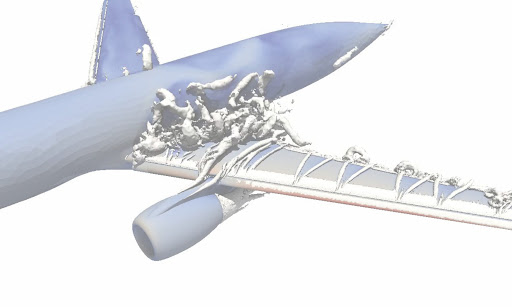
\includegraphics[width=.95\textwidth]{3Dplane.jpg}
	\captionsetup{labelformat=empty}
	\caption{Source: \href{http://www.fenics-hpc.org/}{FEniCS-HPC website}}
\end{figure}





\thispagestyle{empty}

\newpage

\section{Résume du projet}

Le but du projet MORPHEUS consiste à mettre en place des méthodes numériques
pour accélérer la simulation des problèmes d'interaction fluide-structure (IFS), par rapport au temps de calcul requis pour une simulation haute-fidélité. Il sera donc possible d’intégrer des modèles plus économiques, qui pourront remplacer des simulations très coûteuses, et ainsi de faciliter le design optimisé des composant et la prise de décisions. Différemment de plusieurs méthodes proposées dans la littérature, l'impératif est la fidélité à la structure physique du problème.  Cette structure est le plus souvent ignorée par les algorithmes de réduction, qui traitent les simulations comme des boîtes noires. Les modèles réduits respectueux de la physique sont beaucoup plus précis que ceux qui ne la garantissent pas et leur utilisation pourra radicalement améliorer les techniques normalement utilisées pour la réduction des modèles et l'optimisation. Pour realiser son ambition, ce projet vise à utiliser des formalismes mathématiques récents pour la modélisation multiphysique et la digitalisation des modèles. Les outils capables de prédire précisément le comportement des systèmes complexes ont une importance fondamentale pour nous aider à affronter les prochains défis technologiques et sociétaux. Le fait que cette année le Prix Nobel de Physique ait été attribué à trois chercheurs travaillant sur ce sujet\footnote{\url{https://www.nobelprize.org/prizes/physics/2021/summary/}} confirme
l’importance et l'actualité de cet axe de recherche.


\section{Développement du projet scientifique}

\subsection{Les problèmes multiphysiques}
L'ingénierie computationnelle est une science récente, multidisciplinaire et en expansion rapide. Son but consiste à mettre en place des modèles mathématiques et numériques pour prédire le comportement des systèmes complexes. Cela permet d'éviter l'utilisation des tests expérimentales très couteaux pour les systèmes en phase de conception et de détecter de fautes pendant le cycle de vie des composants. Ce domaine est en expansion rapide car aujourd'hui on dispose des ordinateur plus puissant et surtout parce que, grâce au développement des codes open source, les logiciels des calcul sont beaucoup plus accessibles, robustes et faciles à utiliser. Toutefois les problèmes multiphysique, qui sont centrales dans les applications industrielles, sont extrêmement compliqués à traiter. Cela est d\^u d'une part à la difficulté associé au traitement des différentes physique et d'autre part à la taille des systèmes obtenus, qui nécessitent des plusieurs jours, voir plusieurs semaines, pour être résolu à l'aide d'un supercalculateur \cite{keyes2013}. Ces problématiques posent des barrières pour l'utilisation des modèles numériques en industrie. 


\subsection{Outils scientifiques du projet MORPHEUS}

\begin{figure}[tb]
	\centering
	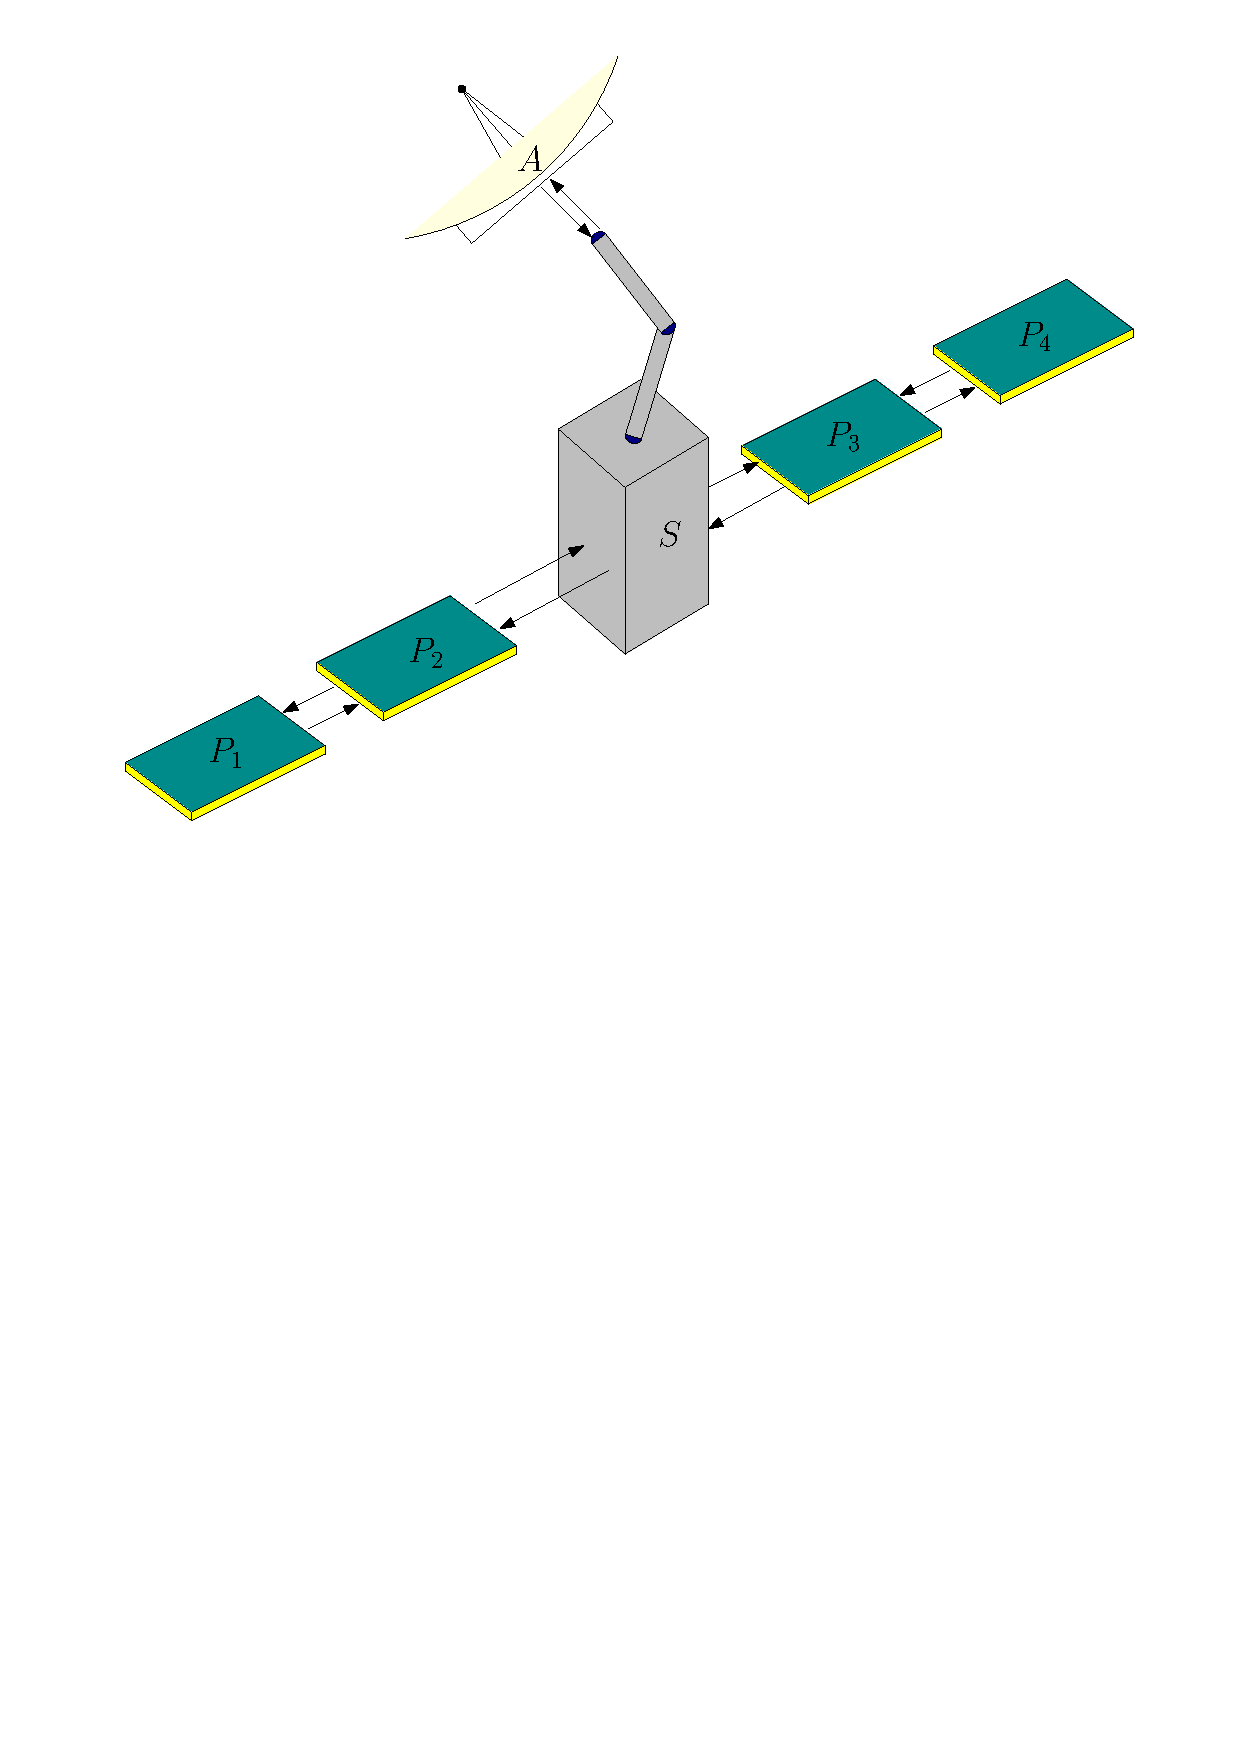
\includegraphics[width=.6\textwidth]{satellite.pdf}
	\caption{Schéma modulaire représentant un satellite de télécommunication.}
	\label{fig:satellite}
\end{figure}

\paragraph{\large Un formalisme unifiant pour la modélisation des systèmes dynamiques\\}
Un formalisme mathématique très prometteur pour traiter les problèmes multiphysique est le formalisme port-Hamiltonienne \cite{vanderSchaft2002}, basé sur la mécanique Hamiltonienne et les graphes de liaisons pour la modélisation des systèmes dynamiques. Au c\oe{}ur de ce formalisme il y a l'idée que tout système physique peut être décrit d'une manière modulaire, c'est a dire à partir des ses composant simples, qui interagissent entre eux et avec le milieu environnant à travers des portes. Les portes d'interactions contiennent l'information relative au flux d'énergie entre les différents composants et entre différents domaines physiques (mécanique, électromagnétisme ou fluidodynamique). La conception modulaire est fondamentale dans l'ingénierie, car le design de tout système technologique est fait à partir des éléments simples qui sont assemblés pour donner lieu à la complexité qui nous entoure. Prenez par exemple un avion, un hélicoptère, un satellite (cf. Fig. \ref{fig:satellite}) ou un téléphone portable : pour pouvoir optimiser leur design il est indispensable de disposer d'un outil de modélisation capable de décomposer la complexité d'une manière à retrouver les différents composants clés. Le fait d’utiliser un outil de modélisation unifié représente une nouveauté essentielle de ce projet. Cela pourra permettre la création d’une infrastructure commune pour les outils numériques à la base de la digitalisation,  et donc faciliter son adoption dans l'industrie.

\paragraph{\large Une methodologie structurée pour la discretisation des EDP\\}
Les algorithmes numériques utilisés en industrie sont adaptés à la nature physique du problème. Pour la mécanique la méthode des éléments finis est privilège par les ingénieur. Pour la fluidodynamique, les volumes finis sont majoritairement utilisés car il garantissent le respect des lois de conservation. Quand il faut utiliser ces deux approches simultanément, par exemple pour traiter des problèmes couplés, leur couplage pose plusieurs challenges. Les deux méthodes utilisent des dégrées de liberté différents (i.e. différents entités topologique du maillage) et l'interconnexion introduit forcement des erreurs. Un outil de modélisation général nécessite d'une méthode de discrétisation également générale, capable de  garantir la possibilité d'interconnecter des physiques distinctes. Ce formalisme unifiant, la méthode des éléments finis en calcul extérieur or FEEC\footnote{Le calcul extérieur représente une généralisation du calcul vectorielle basée sur la géométrie différentielle.},  à été développé récemment \cite{arnold2006acta}. Cette théorie mathématique à permis des développement importants pour la discrétisation des équation à dérivées partielles issues de la physique. Elle à été appliqué avec succès au cas de la mécanique des solides, la fluidodynamique et l'électromagnétisme et elle représente un outil puissant pour les application multiphysique. 

\paragraph{\large L'intelligence artificielle pour obtenir des modeles reduits\\}
Toute méthode de discrétisation, même les plus sophistiquées, amène à des systèmes dont la taille dépasse facilement le million d'inconnus. Pour pouvoir optimiser le design des composantes mécaniques, il faut simuler ces modèles plusieurs fois. Cela amène à des coûts computationnelles prohibitifs même pour les entreprises dotés de plus avancés centres de calcul. Il est donc indispensable d'introduire des méthodes de réduction, qui sont sensé construire un modèle plus simple, capable néanmoins de retenir les propriétés principales du système de départ. La grande majorité de ces méthodes supposent que l'on puisse obtenir un système réduit à travers une méthode essentiellement linéaire, i.e. la Décomposition Orthogonale en Valeurs Propres (POD) \cite{shinde2019,tello2020fluid}. Cette hypothèse n’est pas valable pour tout système exhibant un comportement non-linéaire et conduit à surestimer la dimension du système réduit. Grâce aux progrès récents dans le domaine de l'Intelligence
Artificielle (IA), de nouvelles méthodes permettent d'obtenir des modèles réduits rapides. Récemment, des chercheurs ont proposé une architecture basée sur le réseaux neuronaux convolutifs \cite{lee2020} pour obtenir des modèles beaucoup plus rapide (d'un facteur 100 environ) par rapport aux discrétisation haute fidélité. Leur technique représente une extension non linéaire des méthodologie couramment utilisée. Les résultats obtenus démontrent la gain de performance qu'il est possible obtenir avec cette méthodologie (cf. \ref{fig:deepROM}).

\begin{figure}[t]
	
	\begin{subfigure}[t]{0.465\textwidth}
		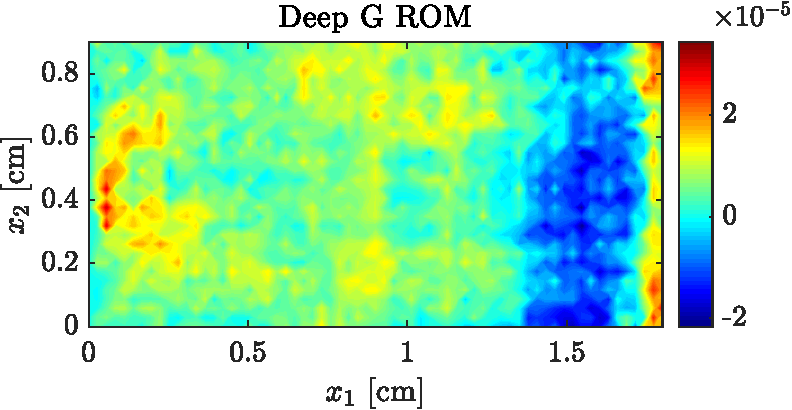
\includegraphics[width=\columnwidth]{DGROM_T_param1.pdf} 
		\caption{Modèle réduit avec réseaux des neurones.}
		\label{fig:DG_ROM}
	\end{subfigure}\hfill
	\begin{subfigure}[t]{0.48\textwidth}
		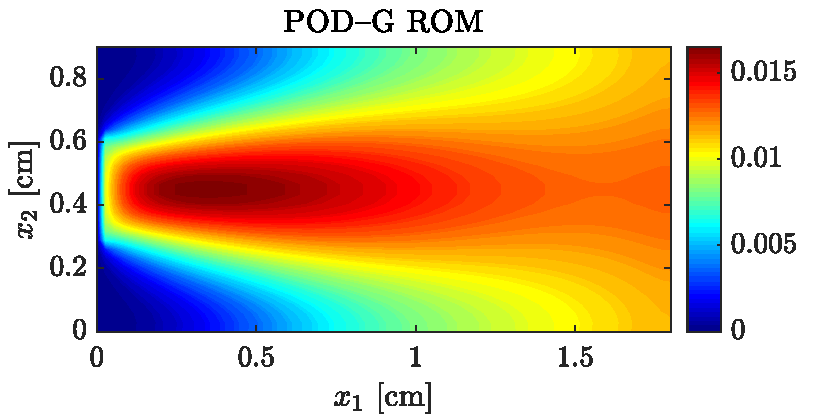
\includegraphics[width=\columnwidth]{GROM_T_param1.pdf}%
		\caption{Modèle réduit avec la méthode linéaire POD.}
		\label{fig:POD_ROM}
	\end{subfigure}
	\caption[]{Erreur des modèles réduits sur le champ de température pour un problème de convection-diffusion-réaction. En utilisant un réseaux neuronaux convolutifs pour générer une variété non linéaire (cf. Fig. \ref{fig:DG_ROM}) l'erreur associé à la réduction  est drastiquement réduit, de $10^{-2}$ à $10^{-5}$, par rapport à la méthode POD (cf. Fig. \ref{fig:POD_ROM}). Reproduit de \cite{lee2020} avec permission.}%
	\label{fig:deepROM}%
\end{figure}


\subsection{Lot de travaux}
Le projet est divisé en trois lots de travaux :

\begin{enumerate}
	\item Développement d'algorithmes numériques haute-fidélité pour des problèmes d'interactions fluide-structures basée sur le formalisme port-Hamiltonien et les élément finis en calcul extérieur.
	\item Méthodes de réduction garantissant le respect de la structure physique générés en utilisant les réseaux des neurones. 
	\item Utilisation des modèles réduits pour l'optimisation et comparaison avec les  modèles haute-fidélité.
\end{enumerate}

Chaque macro-tâche est directement associ\'ee \`a une thèse. Pour ce qui concerne les aspect théoriques fondamentaux Bernhard Maschke (Universit\'e de Lyon), Arjan van der Schaft (University of Groningen) et Stefano Stramigioli (University of Twente) constitueront les interlocuteurs académiques principaux.


\paragraph{\large WP1 : méthodes numériques pour systèmes couplés fluide-structure\\
Responsable: Andrea Brugnoli et Doctorant 1, co-encadré par Denis Matignon (DISC, ISAE)\\}
 Dans ce premier lot de travail, on cherche à obtenir des modèles couplés d'interaction fluide-structure dans le cas où la partie structurelle est considérer déformable. Une fois que ces modèles seront dérivées, le focus principal de ce lot sera de générer des chemins numériques pour la préservations de la structure Hamiltonien à l'aide de la méthode à éléments finis en calcul extérieur. Cette tache représente un véritable défi computationnelle, spécialement si on cherche à résoudre le cas plus général possible d'interaction fluide-structure où la partie mécanique est très flexible et effectue des mouvements rigides. On pourra alors diviser la tache en considérant des problèmes de complexité croissante. 
\begin{enumerate}
	\item Si la structure est encastrée et les déformations sont petits, par exemple une aile d'avion en conditions nominaux, on peut utiliser un maillage fixe au cours du temps. Ceci est du au fait que on peut utiliser les équations linéaire pour l'élasticité. 
	\item Si la structure peut bouger d'une manière rigide mais les déformations restent petites des approches existent pour limiter la complexité des équations.
	\item Dans le cas le plus général, l'élasticité non linéaire doit être considérée. Pour les structures minces, des formulation intrinsèque Hamiltonienne sont déjà disponibles \cite{hodges2003exact}.
\end{enumerate}
Le doctorant devra alors concevoir des méthodes numériques capable de s'adapter à cette complexité croissante. La première défi portera à la résolution du premier cas, qui ne demandera pas d'introduire des technique spéciales pour modifier le maillage. Au contraire le cas successifs devront utiliser des méthodes pour considérer le déplacement du corps élastique (comme par exemple la méthode de frontières immergées \cite{peskin2002}). Ces modèles numériques devront retenir les propriétés physiques du problème (conservation d'énergie globale, traçage des échanges d'énergie entre les différents sous-systèmes, conservation d'invariants du problème).

Pour ce première macro-tâche, il sera possible de prolonger le travail effectué dans le cadre de ma thèse, qui a donn\'e lieu a un code de calcul pour application multiphysique (le code SCRIMP décrit dans \url{https://zenodo.org/record/4945329#.Yd8UJoTMJH4}). Ce code sera ultérieurement développé pour traiter des problèmes d'interaction fluide-structure. Le co-encadrant de thèse sera Denis Matignon, du fait de sa grande expertise concernant les mathématique numérique et les systèmes port-Hamiltonien.

Pour ce qui concerne la préservation de la physique au sein des algorithmes, des collaborations avec Marc Gerritsma (département d'aérodynamique à TU Delft) et Herbert Egger (Johannes Kepler University Linz) seront mises en place. Pour ce qui concerne l'interaction fluide-structure, l'office National d'Études et de Recherches Aérospatiales (ONERA), garant d'une profonde expertise en ce domaine, représentera l'interlocuteur principal pour les problèmes liés au couplage multiphysique.

\paragraph{\large WP2 : réduction de modèles garantissant le respect de la structure physique\\
Responsable: Andrea Brugnoli et Doctorant 2, co-encadré par Charles Poussot-Vassal (ONERA)\\}

Le second challenge du projet consiste à intégrer des techniques issues de l’Intelligence
Artificielle, qui seront utilisées pour obtenir des modèles réduits. Une technique très prometteuse en ce sens est présentée dans \cite{lee2020}, mais ici le respect des lois physiques est imposé a posteriori au travers de contraintes et non pas inclus au niveau de la structure de départ. Dans \cite{sun2020physics} des réseaux de neurones, entraînés pour minimiser l’erreur par rapport au bilan de masse et de la quantité de mouvement, sont utilisés pour s’affranchir de la simulation haute fidélité. Cela ne garantit pas le respect de la structure physique et pose des soucis au niveau de l’interprétabilité des résultats.

Par structure physique du problème on indique la présence des lois de conservation (associé à un opérateur anti-symétrique) et des effets dissipatifs, et les variables qui définissent l'interconnexion entre le fluide et le solide. Conserver la structure physique de la simulation haute fidélité dans la représentation réduite permettra d’intégrer des outils d’intelligence artificielle d’une façon interprétable. Par exemple, des réseaux des neurones peuvent être utilisé pour représenté l'énergie (i.e une fonction entre la dimension de l'état et un scalaire positif), ou l'opérateur associé à la conservation d'énergie, ou bien à sa dissipation. 

Pour ce qui concerne la deuxième macro-tâche, il sera possible de mettre en place des collaboration avec Volker Mehrmann (TU Berlin) et George Haller (ETH Zurich).


\paragraph{\large WP3 : optimisation à l'aide des modèles réduits\\
	Responsable: Andrea Brugnoli et Doctorant 3, co-encadre par Joseph Morlier (MS2M, ISAE) et Post-doc 1\\}

Les techniques développes dans les deux premières lots de travaux permettront d'obtenir des modèles pour décrire l'aéroélasticité et la dynamiques des drones robotiques dans un fluide.
Le dernier objectif consistera à utiliser ces modèles réduits pour l'optimisation. Cette étape permettra d’évaluer la validité et l’efficacité des modèles réduits par rapport aux simulations fines. Selon le cas d'application, différents scénarios ou l'optimisation est nécessaire peuvent être évalués (cf. Fig. \ref{fig:optmisation}): 
\begin{itemize}
	\item L'optimisation structurelle des composant mécaniques en aéronautique, pour augmenter les performances aérodynamiques (minimisation de la traînée et donc la consommation du carburant, cf. Fig. \ref{fig:wing}); 
	\item Co-design de la partie structurelle et du contrôleur embarqué. Cette méthodologie consiste à optimiser le performance du contrôleur (qui cherche par exemple à limiter les vibrations), au même temps que les caractéristiques structurelles du véhicule (par exemple la masse ou la rigidité). Ce type d'optimisation est souvent utilisé pour les satellites (cf. Fig. \ref{fig:codesign_sat}).
	\item Contrôle optimal pour suivi de trajectoire. Ce type des problématiques apparaissent fréquemment en robotique. Les chercheurs s'intéressent de plus en plus à la robotique molle (soft robotics en anglais, cf. Fig. \ref{fig:sofi-mit}), ou la flexibilité des composants ne peut pas être négligée.
\end{itemize}

Typiquement dan l'industrie l'optimisation et les études paramétriques sont effectuées sur les
modèles de substitution, car optimiser directement les modèle fines amène à des coûts computationnelles absolument prohibitifs. Venir à bout de ces trois macro-tâches
permettra de mieux comprendre le compromis entre temps de calcul et précision pour des
applications d’intérêt industriel. Potentiellement, les techniques développées dans ce projet pourront fournir des solutions plus performantes que celles normalement utilisées en industrie. Pour cette tache un doctorant et un chercheur doctoral seront embauchés. 

\begin{figure}[t]
	\begin{subfigure}[t]{0.3\textwidth}
		\includegraphics[width=\columnwidth]{MDo_wing.png}%
		\caption{Optimisation multidisciplinaire d'une aile: rouge design optimise (reproduit avec permission de \cite{masColomer2021mdo}). }
		\label{fig:wing}
	\end{subfigure}\hfill
	\begin{subfigure}[t]{0.3\textwidth}
		\includegraphics[width=\columnwidth]{Codesign_satellite.pdf} 
		\caption{Modèle d'un satellite pour le co-design contrôle/structure (reproduit avec permission de \cite{finozzi2022sub})}
		\label{fig:codesign_sat}
	\end{subfigure}\hfill
	\begin{subfigure}[t]{0.35\textwidth}
		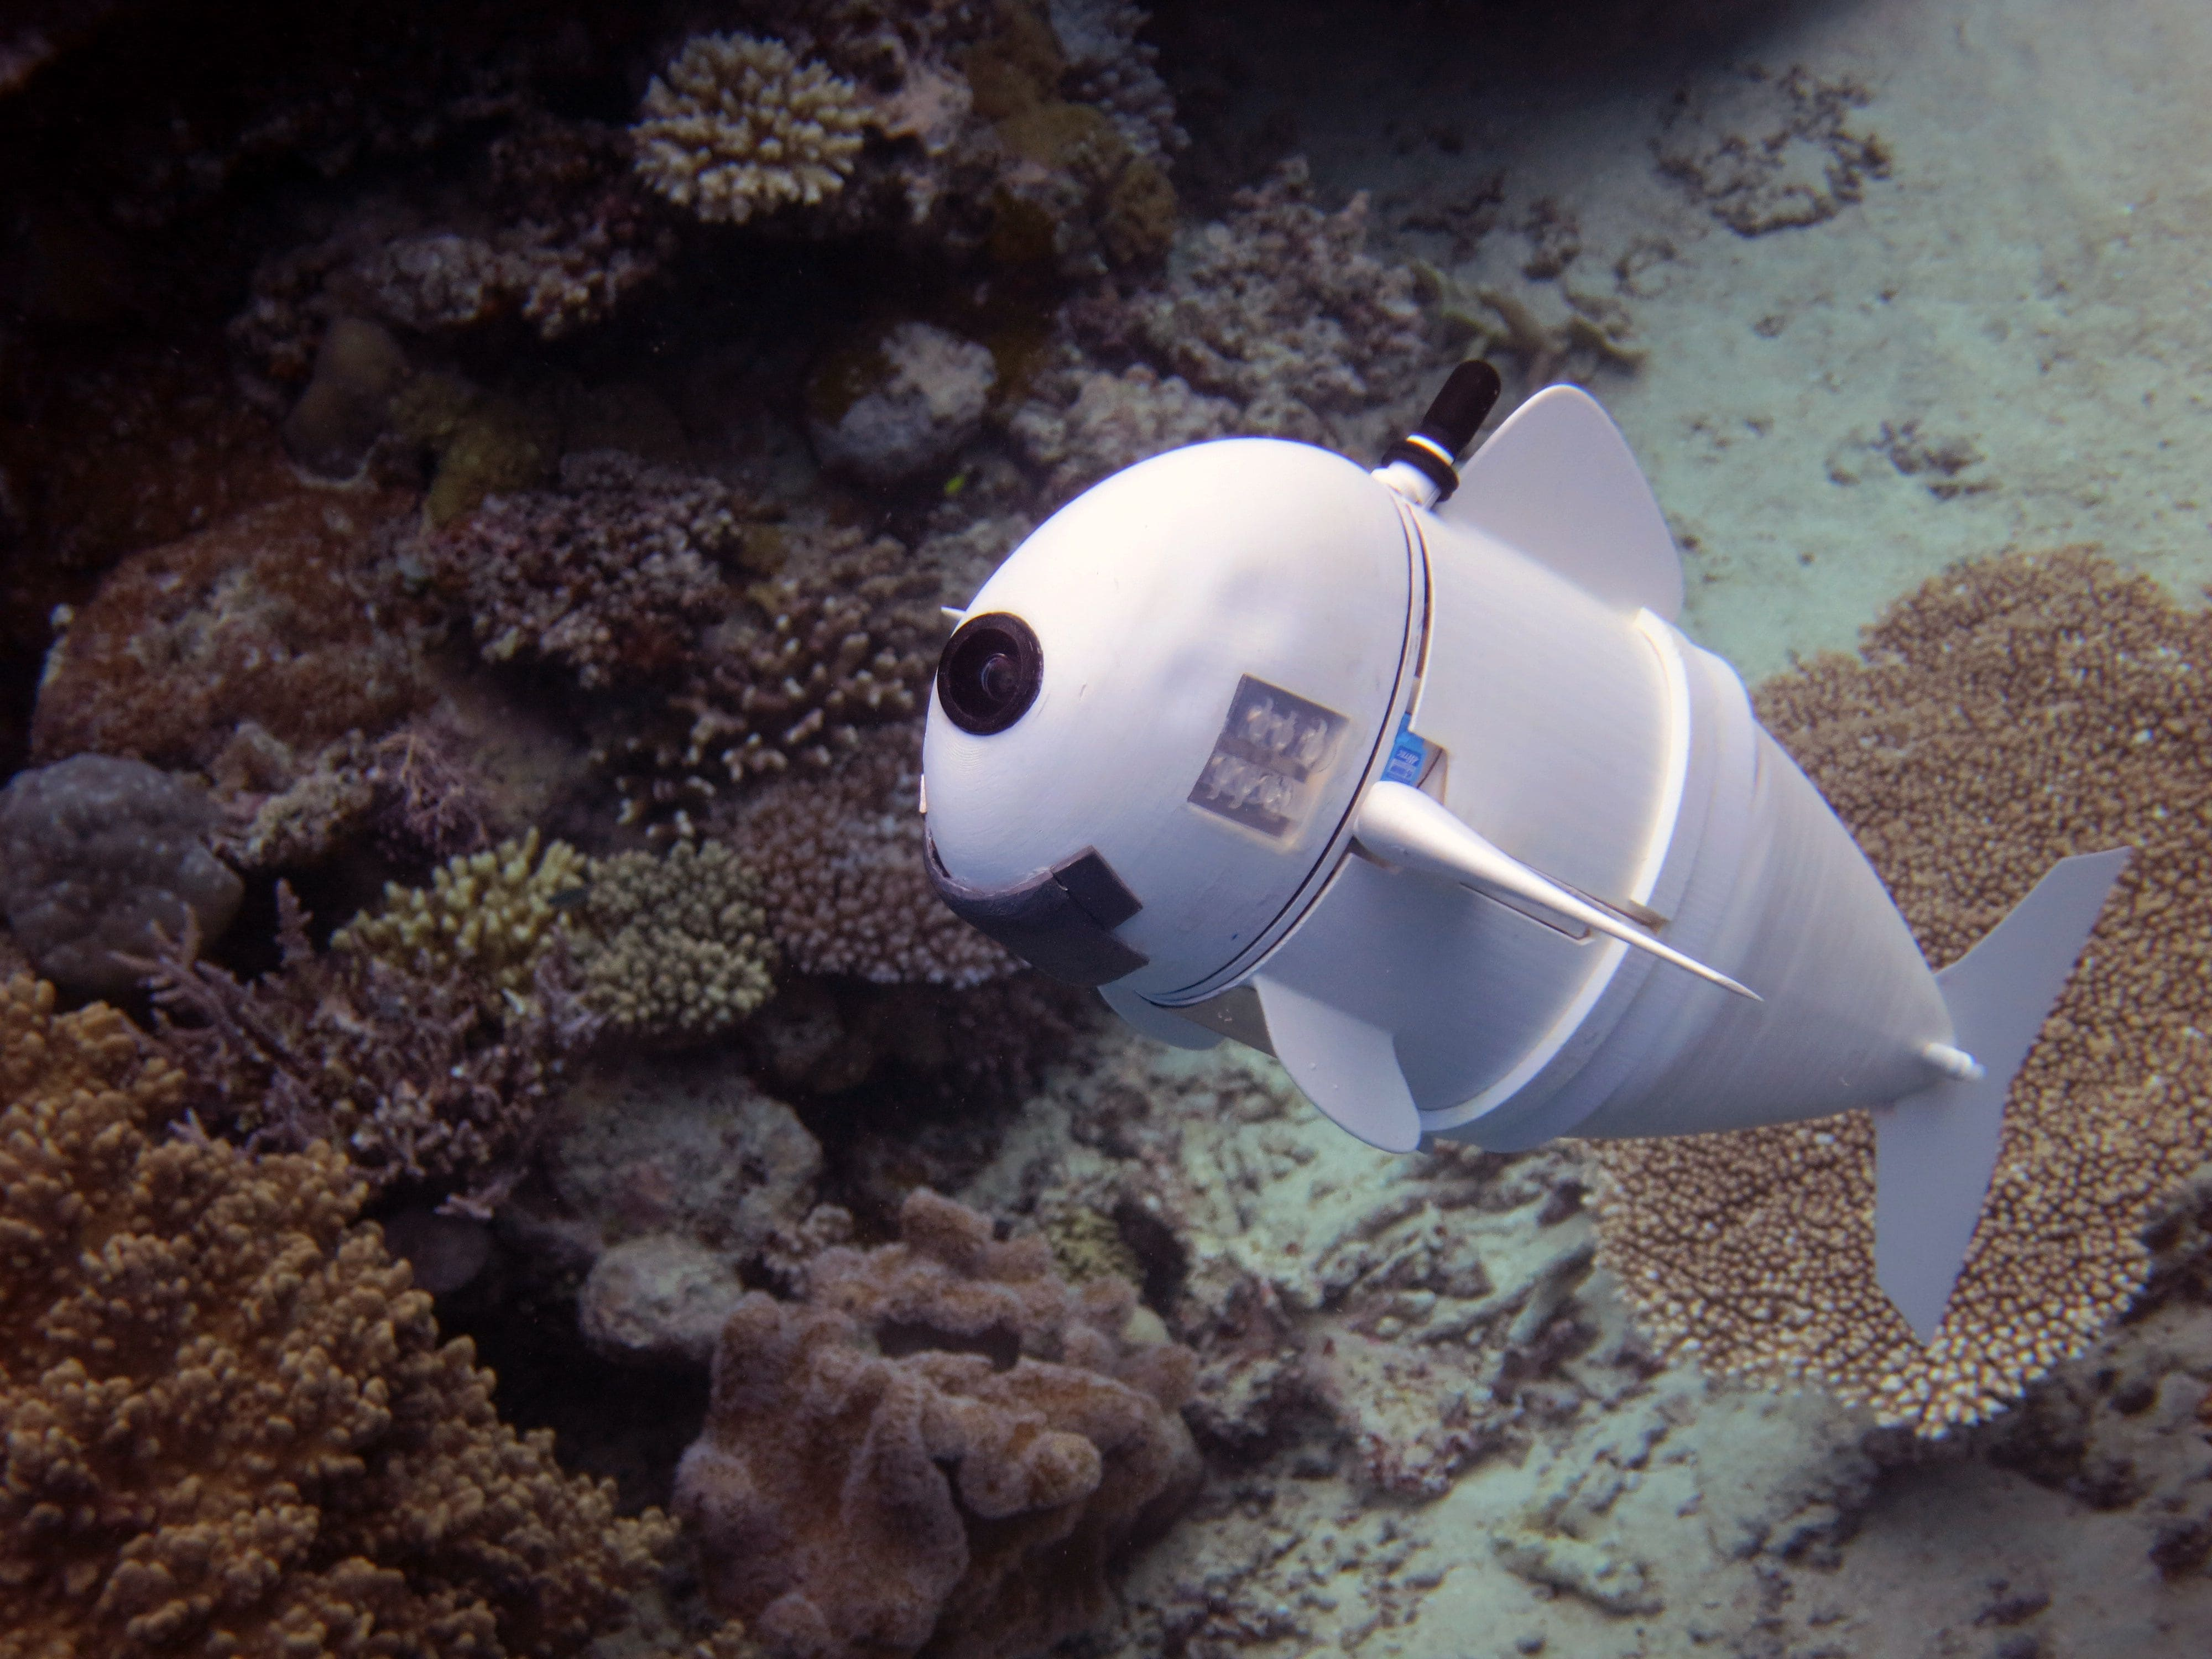
\includegraphics[width=\columnwidth]{Sofi_MIT.jpeg}%
		\caption{Le drone robotique Sofi du MIT (\href{https://www.csail.mit.edu/research/sofi-soft-robotic-fish}{Lien à la page web})}
		\label{fig:sofi-mit}
	\end{subfigure}
	\caption[]{Cas d'application pour les problèmes optimisation dans la WP3.}%
	\label{fig:optmisation}%
\end{figure}


\section{Mise en \oe{}vre du projet}

\subsection{Objectifs et échéances}

Le travail sera effectuer au sein du département DISC de l'ISAE. Pour ce qui concerne son développement, les objectifs suivant seront considérés.

\begin{itemize}
	\item \textbf{De T0 à T0 + 6 mois :} Création des partenariat académiques et industriels.
	Pour ce qui concerne l'architecture logiciel pour le calcul haute performance, on cherchera à organiser la première thèse en collaboration avec le CEA (centre pour l'énergie atomique). Cette structure possède l'un de centre de calcul plus sophistiqué de France. Il est donc logique d'envisager la création d'une thèse en cotutelle avec cette institution. On cherchera également d'effectuer de collaboration avec Airbus, spécialement pour ce qui concerne la partie optimisation.
	\item \textbf{De T0 + 6 mois à T0 + 12 mois : } Recrutement du première doctorat, chargé du premier lot de travail. Cette thèse sera effectuer en cotutelle avec le CEA. Le doctorant devra avoir des compétence en mathématiques appliquées et modèles pour l'ingénierie. Cette thèse aura comme but la génération d'un code multiphysique pour la mécanique et la fluidodynamique.
	\item \textbf{De T0 + 12 mois à T0 + 18 mois : } Recrutement du deuxième doctorant, en collaboration avec Charles Poussot-Vassal et l'Onera. Pour cette thèse, on cherchera un doctorant avec des compétences en calculs scientifique et Intelligence Artificielle. Cette thèse sera organisée en sort que les modèles générés dans le WP1 puissent être utilisés par le doctorant 2.
	\item \textbf{De T0 + 18 mois à T0 + 24 mois : } Recrutement du troisième doctorant. Pour cette thèse, on cherchera un profile ingénieur avec des compétences solides en mécanique. Ce thésard travaillera avec le département MS2M de l'ISAE. Il sera possible d'organiser cette thèse en collaboration avec AIRBUS.
	\item \textbf{De T0 + 24 mois à T0 + 30 mois : } Recrutement d'un chercheur doctoral. La personne embauchée sera expert en utilisation de l'intelligence artificielle pour l'optimisation et accompagnera le thésard 3. 
	\item \textbf{De T0 + 36 mois à T0 + 42 mois : } Mise en forme du logiciel de calcul développé dans le WP1. Création de la documentation pour le code et des tutoriaux pour son utilisation.
	\item \textbf{De T0 + 48 mois à T0 + 54 mois : } Validation du code pour la réduction de modèles pour les problèmes d'interaction couplés.
	\item \textbf{De T0 + 54 mois à T0 + 60 mois : } Finalisation du code de calcul, regroupant la génération des modèles haute-fidélité, la réduction de modèles et l'optimisation. Dissémination des résultats.
\end{itemize} 

\begin{figure}[h!]
	\begin{center}
		\begin{ganttchart}[y unit title=0.6cm,
			y unit chart=0.6cm, 
			x unit=0.4cm,
			vgrid,hgrid, 
			title label anchor/.style={below=-1.6ex},
			title left shift=.05,
			title right shift=-.05,
			title height=1,
			progress label text={},
			bar height=0.7,
			group right shift=0,
			group top shift=.6,
			group height=.4]{1}{30}
			%labels
			\gantttitle{Dur\'ee totale}{30} \\
			\gantttitle{$T_0 + 12$}{6} 
			\gantttitle{$T_0 + 24$}{6} 
			\gantttitle{$T_0 + 36$}{6} 
			\gantttitle{$T_0 + 48$}{6} 
			\gantttitle{$T_0 + 60$}{6} \\
			%tasks
			\ganttbar{Partenariats}{1}{2} \\
			\ganttbar{Code SCRIMP}{1}{1} \\
			\ganttbar{1$^\circ$ th\`ese}{4}{21} \\
			\ganttbar{2$^\circ$ th\`ese}{10}{27} \\
			\ganttbar{3$^\circ$ th\`ese}{13}{30} \\
			\ganttbar{Post-Doc}{16}{27} \\
			\ganttbar{Soutenances}{22}{30} \\
			\ganttbar{Dissémination}{28}{30} 
			%relations 
			\ganttlink{elem0}{elem2} 
			\ganttlink{elem1}{elem2} 
			\ganttlink{elem1}{elem3} 
			\ganttlink{elem1}{elem4} 
			\ganttlink{elem1}{elem5}
			\ganttlink{elem2}{elem5}
			\ganttlink{elem3}{elem5}
		\end{ganttchart}
	\end{center}		
\end{figure}


\subsection{Choix de l'institution d'accueil}
Pour ce projet, on choisi l'ISAE et sa grande expertise dans le domaine aéronautique. En effet les applications aéronautiques sont centrales dans ce projet. En plus, l'intégration des compétences diverses au sein de l'institution permettra le dialogue entre experts dans les différentes disciplines requises : calcul numérique et intelligence artificielle (département DISC), aérodynamique (DAEP) réduction de modèles (DCAS), optimisation structurelle (MS2M).


\subsection{Budget}


\begin{center}
\begin{tabular}{|c|c|}
	\hline
	D\'epense & Co\^{u}t \\
	\hline
	Porteur du projet (temps plein) & $5\times 60000=300000$ \\
	3 doctorants (temps plein) & $3\times 3\times 40000=360000$  \\
	1 Post-Doc (temps plein) & $2\times 55000=110000$ \\
	Personnels ISAE & $100000$ \\
	Matériel  et calcul HPC & $60000$ \\
	Frais annexes (conférences, workshops) & $60000$ \\
	\hline
	\textbf{Total} & 1000000 \\
	\hline
\end{tabular}
\end{center}

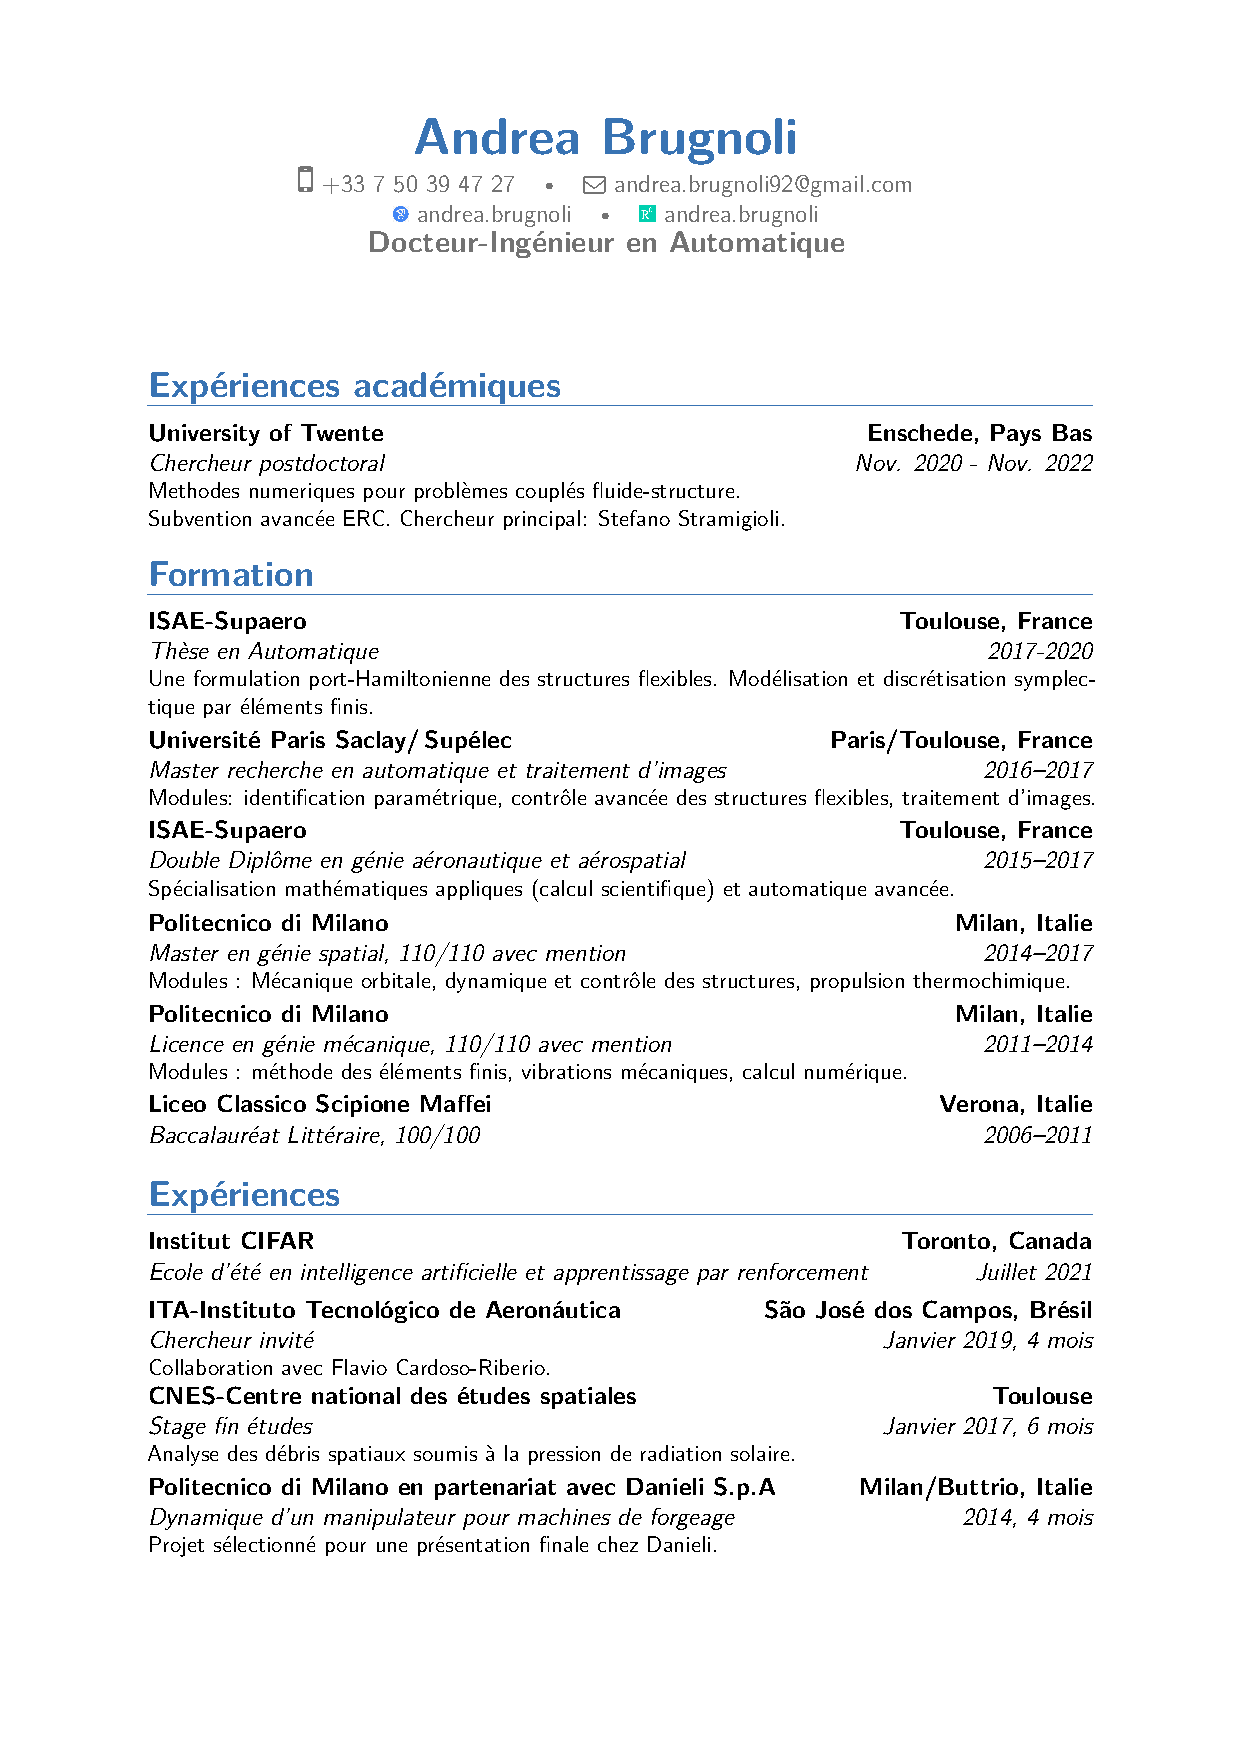
\includepdf[pages=-]{cv_french.pdf}

\section{Plan de carrière}

La technologie, les sciences et leur impact sur l'humain m'ont toujours intéressé. C'est pour cela que j'ai effectué mes études en ingénierie dans des institutions prestigieuses (double diplôme Politecnico di Milano et ISAE-SUPAERO et master de recherche en collaboration avec Supélec/Université Paris Saclay). Mes études ont été centrés sur le calcul numérique, les systèmes dynamiques et l'automatique. Mon intérêt pour la simulation des problèmes physiques m'a amené au centre national d'études spatiales (CNES) pour mon stage de fin études. \\

L'ISAE a financé le projet de thèse pour le quel j'avais été sélectionné. Dans ce travail, j'ai exploré le potentiel d'un formalisme mathématique pour la modélisation des systèmes mécaniques complexes. J'ai pu développer des compétences à l'intersection des mathématiques appliques, physique et ingénierie des systèmes. La révolution digitale qui est en cours maintenant donne aux ingénieurs des instruments puissants pour pousser les avancés technologiques. Je considère l'expertise acquise pendant la thèse comme fondamentale, car maintenant je possède les compétences nécessaires pour être acteur de cette révolution. Cette même expertise m'a permit d'être sélectionné comme chercheur doctoral dans un projet ERC à l'université de Twente. Ce projet est extrêmement passionnant car il réuni différents chercheurs travaillant dans les aspects théoriques et/ou pratiques de la robotique pour perfectionner le design d'un drone bio-inspire. \\

\`A moyen terme je souhaite postuler comme ingénieur de recherche ou maître de conférence dans une Université ou Laboratoire en France. Je souhaite continuer à travailler dans la modélisation mathématique pour l'ingénierie, en travaillant entre les mathématiques appliquées et l'informatique. Mon idéal serait de travailler dans un organisme qui cherche à résoudre des problèmes d'intérêt sociétal, en utilisant les outils de l'ingénierie computationnel.  Si le projet MORPHEUS sera sélectionné pour le prix Lopez-Loreta, je me consacrerai au plein temps à sa réalisation. Ce projet touche à différentes thématiques qui sont centrales dans mes intérêts. La possibilité de pouvoir le financer pendant 5 ans représente une opportunité unique de croissance professionnelle. J'envisage de soutenir une Habilitation à diriger des recherches dans un horizon de 10 ans.


\section{Production scientifique}
{
\nocitearticle{brugnoli2019ammmin,brugnoli2019ammkir,brugnoli2020msd,brugnoli2021ther,brugnoli2021num,califano2021}
\bibliographystylearticle{unsrt}
\bibliographyarticle{biblio_articles}

\nociteconf{brugnoli2019cpde,brugnoli2019cdc,cardoso2019cdc,brugnoli2020wc,brugnoli2020mtns,brugnoli2021vk,cherifi2021data,rashad2021ext}
\bibliographystyleconf{unsrt}
\bibliographyconf{biblio_conf}  
 
\nociteconfnoproc{brugnoli2021siamcse}
\bibliographystyleconfnoproc{unsrt}
\bibliographyconfnoproc{biblio_confnoproc}   
}



\bibliographystyle{unsrt}
\bibliography{biblio_dossierLL}


\end{document}
